\documentclass[12pt,a4paper]{article}

\usepackage{style2017}
\newcounter{numexo}
\setcellgapes{1pt}
% Modification espace après paragraphe +6pt
\parskip=5pt

\begin{document}


\begin{NSI}
{Activité}{Dictionnaires}
\end{NSI}

%\section*{Introduction}

Un \textbf{dictionnaire} est une structure de données qui permet de mémoriser et d'enregistrer des données en utilisant des associations entre des \textbf{clefs} et des \textbf{valeurs}.

\begin{itemize}[label=\textbullet]
\item Une \textsf{clef} est une chaine de caractères, type \textsf{string}. Chaque \textsf{clef} du dictionnaire est \textbf{unique}. Cette unicité garantit l'accès à la valeur associée.

\item La \textsf{valeur} associée à une \textsf{clef} peut de tout type : nombre \textsf{int} ou \textsf{float}, une chaine de caractères \textsf{string}, un booléen \textsf{bool}, un tableau \textsf{list} ou \textsf{tuple} et même un dictionnaire \textsf{dict}.
\end{itemize}

L'ordre est important dans la notation. En premier, on écrit la \textsf{clef}, en second, la \textsf{valeur} associée à la clef.

En python, un \textbf{dictionnaire} est une structure de données native notée entre \textbf{accolades}. 

Un dictionnaire est créé:

\begin{itemize}[label=\textbullet]
\item soit avec la fonction \textsf{dict()};

\item soit en énumérant les clefs et les valeurs sous forme de paire \textsf{'clef' : valeur}, le tout noté entre des \textbf{accolades}, les différentes paires étant séparées par des virgules.
\end{itemize}

\textbf{Quelques exemples de création de dictionnaires:}

\begin{center}
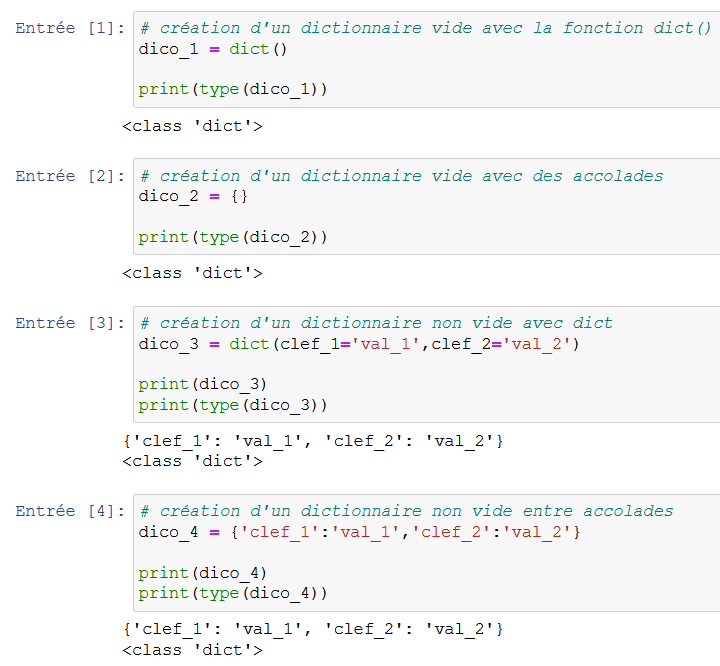
\includegraphics[scale=0.8]{img/creer_dictionnaire.png}
\end{center}

\section*{Créer des dictionnaires}

\begin{enumerate}
\item Notre premier dictionnaire contient les chiffres du système décimal. Chaque clef est le chiffre écrit en lettre et chaque valeur et le chiffre lui-même. Par exemple, pour le chiffre zéro, la clef est \textsf{zéro} et la valeur \textsf{0}.

\begin{enumerate}
\item Créer un dictionnaire vide \textsf{chiffres}.
\item L'ajout d'une donnée dans un dictionnaire suppose d'insérer une nouvelle clef et la valeur associée. La syntaxe est : \textsf{chiffres['clef'] = valeur}.

Ajouter au dictionnaire \textsf{chiffres} les dix chiffres du système décimal.

\item Compléter le dictionnaire \textsf{chiffres} pour avoir tous les chiffres du système hexadécimal.
\end{enumerate}

\item Notre second dictionnaire contient les capitales de pays européens. Chaque clef est un nom de pays et la valeur associée est une capitale.

\begin{enumerate}
\item Créer un dictionnaire \textsf{pays\_capitales} contenant 5 pays européens avec leurs capitales.
\item Ajouter deux pays européens et leurs capitales.
\end{enumerate}
\end{enumerate}


\section*{Fonctions et méthodes d'un dictionnaire}

Certaines fonctions vues avec les tableaux en Python (liste et tuple) s'appliquent aussi aux dictionnaires.

\begin{enumerate}
\item La fonction \textsf{len} renvoie le nombre d'éléments d'un dictionnaire.

Écrire une instruction python donnant le nombre de valeurs des deux dictionnaires créés précédemment.

\item Les fonctions \textsf{min} et \textsf{max} s'appliquent-elles aux dictionnaires ?

\item Il existe des méthodes propres aux dictionnaires. En voici quatre:

\begin{itemize}[label=\textbullet]
\item La méthode \textsf{keys()} renvoie les clefs d'un dictionnaire; Le type renvoyé est objet itérable, ce qui permet de parcourir son contenu avec une boucle.

\item La méthode \textsf{values()} renvoie les valeurs d'un dictionnaire; Le type renvoyé est objet itérable, ce qui permet de parcourir son contenu avec une boucle.

\item La méthode \textsf{items()} renvoie les paires clefs et valeurs d'un dictionnaire; Le type renvoyé est objet itérable, ce qui permet de parcourir son contenu avec une boucle.

\item La méthode \textsf{get(clef)} prend en paramètre une clef du dictionnaire et renvoie la valeur associée à cette clef.
\end{itemize}

Écrire des instructions en Python pour:
\begin{enumerate}
\item afficher les clefs du dictionnaire \textsf{chiffres}.
\item afficher les valeurs du dictionnaire \textsf{pays\_capitales}.
\item afficher les items du dictionnaire \textsf{pays\_capitales}.
\item afficher les chiffres impairs du dictionnaire \textsf{chiffres}.
\end{enumerate}

\end{enumerate}

\newpage
\section*{Manipuler un dictionnaire}

Le fichier \textsf{capitales.py} contient les différents pays du monde et leurs capitales réunis dans un même dictionnaire. Pour utiliser ce dictionnaire, vous devez enregistrer ce fichier dans le même dossier que votre fichier de travail, puis réaliser un \textsf{import}.

\begin{enumerate}
\item Importer le dictionnaire \textsf{capitales} en saisissant l'instruction python suivante:

\textsf{from capitales import capitales}

\item Combien de données contient le dictionnaire \textsf{capitales} ?

\item Écrire une instruction python qui affiche la capitale du \textbf{Belize}.

\item Écrire un script Python qui permet d'obtenir le pays dont la capitale est \textbf{Port Moresby}.

\item On veut créer un tableau \textsf{Pays\_P} contenant tous les pays commençant par la lettre \textsf{P}. Écrire un script python qui crée ce tableau (attention ce n'est pas un affichage mais une variable).

\item On veut créer un tableau \textsf{Capitales\_C} contenant toutes les capitales commençant par la lettre \textsf{C}. Écrire un script python qui crée ce tableau.

\item On veut créer un tableau \textsf{Pays\_C} contenant tous les pays dont la capitale commence par la lettre \textsf{C}. Écrire un script python qui crée ce tableau (attention ce n'est pas un affichage mais une variable).

\item Écrire une fonction \textsf{recherche} avec 2 paramètres \textsf{nature} et \textsf{lettre}. Le paramètre \textsf{nature} accepte deux valeurs qui sont \textsf{pays} ou \textsf{capitale}. Le paramètre \textsf{lettre} prend comme valeur une \textsf{lettre} de l'alphabet. La fonction renvoie une liste contenant toutes les valeurs (pays ou capitales) commençant par la lettre passée en argument.


\item Certains pays ont un nom de capitale identique au nom du pays. Écrire un script python qui crée une liste contenant ces pays.
\end{enumerate}

%\section*{Intérêt du dictionnaire}
%
%On a déjà rencontré une structure de donnée qui permet d'avoir plusieurs valeurs dans une même variable : la \textbf{liste} python (tableau).
%
%L'accès aux valeurs d'une liste se fait avec la position de la valeur dans la liste par son \textbf{indice}. 
%
%L'accès aux valeurs d'un dictionnaire se fait par les mots clefs. La clef est elle même une variable avec une valeur unique. Cela représente donc un premier intérêt. On va en voir d'autres.

%\subsection{Listes ou dictionnaires}
%On va comparer notre dictionnaire avec une structure de liste. 
%
%On a notre variable \textbf{capitales} de type dictionnaire:
%\begin{lstlisting}
%capitales={
%	'france':'paris',\
%	'italie':'rome',\
%	'espagne':'madrid',\
%	'suisse':'geneve'
%}
%\end{lstlisting}
%On crée une variable \textbf{capitaliste} de type liste comprenant les pays et les capitales de notre dictionnaire.
%On a une liste qui ressemble à :
%\begin{lstlisting}
%capitaliste=[
%	['france','paris'],\
%	['italie','rome'],\
%	['espagne','madrid'],\
%	['suisse','geneve']
%]
%\end{lstlisting}
%\begin{enumerate}
%\item On veut créer une variable \textbf{pays} de type liste contenant tous les pays.
%\begin{enumerate}
%\item Compléter la variable \textbf{pays} en utilisant le dictionnaire;
%\item Recommencer en utilisant la liste;
%\end{enumerate} 
%\item Créer la variable \textbf{villes} de type liste contenant toutes les capitales.
%\item Dans l'interpréteur, modifier la capitale de la Suisse dans nos deux variables \textbf{capitaliste} et \textbf{capitales}.
%\end{enumerate}
%
%\subsection{Plusieurs dictionnaires}
%En utilisant plusieurs dictionnaires avec des clefs communes, on peut gérer simplement plusieurs valeurs. 
%
%Supposons que l'on souhaite avoir pour nos pays, en plus des capitales, des informations sur le continent où chaque pays se trouve et sa population en millions d'habitants. 
%
%On peut regrouper ces valeurs dans le même dictionnaire mais la structure ne sera pas simple à manipuler. On peut tirer avantage à utiliser plusieurs dictionnaires.
%
%On va créer un dictionnaire regroupant pour chaque pays sa capitale, un second dictionnaire regroupant pour chaque pays son continent et un troisième contenant le nombre d'habitants en millions de chaque pays.
%
%On donne un tableau qui contient les informations sur certains pays:
%
%\begin{tabular}{*{4}{|C{4cm}}|}\hline
%\textbf{Pays} & \textbf{Capitale} & \textbf{Continent} & \textbf{Population}\\\hline
%France & Paris & Europe & 67\\
%Italie & Rome & Europe & 61\\
%Allemagne & Berlin & Europe & 83\\
%Brésil & Brasilia & Amérique & 211\\
%Argentine & Buenos Aires & Amérique & 45\\
%Sénégal & Dakar & Afrique & 16\\
%République du Congo & Brazzaville & Afrique & 5\\
%Maroc & Rabat & Afrique & 36\\
%Inde & New Dheli & Asie & 1366\\
%Chine & Pekin & Asie & 1398\\
%Australie & Camberra & Océanie & 25\\\hline
%\end{tabular}
%
%\begin{enumerate}
%\item Créer trois dictionnaires \textbf{capitale}, \textbf{continent} et \textbf{population} contenant les différentes données du tableau. Les clefs de dictionnaires sont les noms de pays.
%\item Écrire un script en Python qui affiche pour un pays donné sa capitale, le continent et sa population.
%\item Créer un script en Python qui ajoute la Suisse aux différent dictionnaires.
%\item Certains pays ont un littoral (accès direct à la mer ou océan). On souhaite ajouter cette information à nos différents pays. Ajouter cette information pour chaque pays dont les valeurs sont des booléens.
%\end{enumerate}
\end{document}

